% Template for Cogsci submission with R Markdown

% Stuff changed from original Markdown PLOS Template
\documentclass[10pt, letterpaper]{article}

\usepackage{cogsci}
\usepackage{pslatex}
\usepackage{float}
\usepackage{caption}

% amsmath package, useful for mathematical formulas
\usepackage{amsmath}

% amssymb package, useful for mathematical symbols
\usepackage{amssymb}

% hyperref package, useful for hyperlinks
\usepackage{hyperref}

% graphicx package, useful for including eps and pdf graphics
% include graphics with the command \includegraphics
\usepackage{graphicx}

% Sweave(-like)
\usepackage{fancyvrb}
\DefineVerbatimEnvironment{Sinput}{Verbatim}{fontshape=sl}
\DefineVerbatimEnvironment{Soutput}{Verbatim}{}
\DefineVerbatimEnvironment{Scode}{Verbatim}{fontshape=sl}
\newenvironment{Schunk}{}{}
\DefineVerbatimEnvironment{Code}{Verbatim}{}
\DefineVerbatimEnvironment{CodeInput}{Verbatim}{fontshape=sl}
\DefineVerbatimEnvironment{CodeOutput}{Verbatim}{}
\newenvironment{CodeChunk}{}{}

% cite package, to clean up citations in the main text. Do not remove.
\usepackage{cite}

\usepackage{color}

% Use doublespacing - comment out for single spacing
%\usepackage{setspace}
%\doublespacing


% % Text layout
% \topmargin 0.0cm
% \oddsidemargin 0.5cm
% \evensidemargin 0.5cm
% \textwidth 16cm
% \textheight 21cm

\title{Preserved Structure Across Vector Space Representations}

\usepackage[utf8]{inputenc}
\usepackage[export]{adjustbox}

\author{{\large \bf Andrei Amatuni, Elika Bergelson} \\ \texttt{\{andrei.amatuni, elika.bergelson\}@duke.edu} \\ 417 Chapel Dr. Durham, NC 27708 USA \\ Department of Psychology and Neuroscience \\ Duke University}

\begin{document}

\maketitle

\begin{abstract}
Certain concepts, words, and images are intuitively more similar than
others (dog vs.~cat, dog vs.~spoon), though quantifying such similarity
is notoriously tricky. Indeed, this kind of computation is likely a
critical part of learning the category boundaries for words within a
given language. Here, we use a set of items (n= 27, e.g. `dog') that are
highly common in young infants' input, and use both image-based and
word-based algorithms to independently compute similarity among these
items. We find two key results. First, the pair-wise item similarities
derived within image-space and word co-occurrence-space are correlated,
suggesting evidence of preserved structure among these extremely
different representational formats. Second, the `closest' neighbors for
each item computed within each space overlap significantly. We further
discuss the potential role of animacy in a set of exploratory analyses.
We conclude that this approach, which does not rely on human ratings of
similarity, may nevertheless reflect stable within-class structure
across these two spaces. We speculate that such invariance, in turn,
might aid in lexical acquisition, by serving as an informative marker of
category boundaries.

\textbf{Keywords:}
vector space models; semantic similarity; word learning
\end{abstract}

\section{Introduction}\label{introduction}

Infants are presented with a challenge to carve the world into distinct
lexical entities in the process of learning their first language.
They're provided with little supervision while mapping a territory which
William James (1890) dubbed a ``great blooming, buzzing confusion''. How
they determine which aspects of the world to attend to in service of
this goal, is an area of ongoing research (Mareschal \& Quinn, 2001).
Different features of objects and their environments are varyingly
informative with regards to object segmentation and category structure.
Some researchers have suggested that categorization is along
fundamentally perceptual grounds and that only later in development is
conceptual knowledge incorporated into these nascent perceptual
categories (Quinn \& Eimas, 1997, 2000; Quinn, Johnson, Mareschal,
Rakison, \& Younger, 2000). Others suggest that there are in fact two
distinct processes at work, such that perceptual categories are computed
automatically by the sensory systems, while conceptual categories are
independently formed through conscious action (Mandler, 2000). Träuble
and Pauen (2007) provide evidence of functional information (regarding
the animacy of objects) influencing early category judgements. Gelman
and Markman (1986) explicitly set these two sources of category cues
against each other (i.e.~functional vs.~perceptual), and find that
preschoolers can override perceptual overlap in reasoning about
functional similarity, in natural kinds. \textbf{add some smith, waxman
refs}

The degree to which conceptual and perceptual information are separable,
both in early learning, and in adult experts, is an important open
question. Any model which hopes to explain the mechanics of human
categorization must address how these potentially disparate
information-sources interface in mental representations, and to what
degree they interact. While evidence from human learners suggests they
integrate perceptual and linguistic information during categorization
and learning (\textbf{REFS}), here we take first steps in a deliberately
different approach. We separate computations over images and words, and
then compare the overlap in the similarity among items that these
systems deduce. Using a set of highly familiar and common words and
concepts from a large infant corpus, we compare the output of an image
analysis, and a word co-occurrence analysis for these same items. We use
algorithms that learn feature representations without hand engineering,
purely as a byproduct of their particular (and separate) training
objectives (e.g.~natural language processing or object recognition in
images). Comparing the representations these algorithms learn, we gain a
window into the structure of visual and semantic forms.

\section{Methods}\label{methods}

\subsection{Items}\label{items}

The 27 items (i.e.~words and images) analyzed here were selected due to
their high frequency in infants' early visual and linguistic input,
aggregated as part of the SEEDLingS project, which gathered longitudinal
audio and video data of infants' home environments from 6-17 months (E.
Bergelson, 2016a, 2016b). We describe this larger study in brief, simply
to relay how the items we analyze were chosen; the details of this
larger study are not critical to the present work. In the larger study,
44 infants were tested every other month (from 6-18 months) on common
nouns, using a looking-while-listening eyetracking design in which two
images are shown on a screen, and one is named. The words for these
experiments were chosen by dint of being high frequency or well known
across infants in other samples (e.g.~Brent Corpus, WordBank (Brent \&
Siskind, 2001; Frank, Braginsky, Yurovsky, \& Marchman, 2017)), or by
being one of the top 10 concrete nouns heard in each infants' own home
audio and video recordings in the preceding two months.

The images displayed when these words were tested were chosen from a
library of prototypical images of a given word (e.g.~dog), along with
images of infants' own versions of the items, as seen in their home
videos (e.g.~a given infant's cat, specific bottle, etc.). To enter the
current analysis, images had to occur 9 or more times in this image
library of high frequency concrete nouns \textbf{add M(SD) R for images
and words in allbasiclevel}. Thus, the words and images used here were
highly common across our 500+ daylong audio-recordings and 500+ hourlong
video-recordings from 44 infants, providing an ecologically-valid
item-set for present modeling purposes.

The images of the 27 items used to derive average category image-vectors
were all 960x960pixel photos of a single object on a gray background.
All items correspond to words found on WordBank (Frank et al., 2017), a
compilation of the MacArthur-Bates Communicative Development Inventory,
which we use as a proxy for age of acquisition below (Dale \& Fenson,
1996).

\subsection{Vector Representations}\label{vector-representations}

We generate two sets of vector representations for a common set of
early-learned items. The first set of vectors are taken from a
pretrained set of GloVe representations (Pennington, Socher, \& Manning,
2014), a modern distributional semantic vector space model. The second
set is taken from the final layer activations of a pretrained image
recognition model, Google's Inception V3 convolutional neural network
(Szegedy, Vanhoucke, Ioffe, Shlens, \& Wojna, 2016). Both of these
representations are generally referred to as ``embeddings''. They map
objects from one medium (e.g.~images or words) into a metric space where
distances between points can be computed and function as a measure of
similarity between objects.

\subsubsection{Word Vectors}\label{word-vectors}

In the case of our word vectors, the GloVe algorithm instantiates the
distributional hypothesis, which proposes that words which co-occur with
each other share similar meaning (Firth, 1957; Harris, 1954), whereby
capturing the covariance of tokens in large text corpora, captures
aspects of their semantic structure. We use the set of vectors
pretrained by the GloVe authors on the Common Crawl corpus with 42
billion tokens, resulting in 300 dimensional vectors for 1.9 million
unique words\footnote{\url{https://nlp.stanford.edu/projects/glove/}}.
Such vectors have shown promise in modeling early semantic networks
(Amatuni \& Bergelson, 2017). Thus, in word-vector space, each of our 27
items is represented as a 300-dimensional vector, with each word
assigned a unique point in a common vector space.

\subsubsection{Image Vectors}\label{image-vectors}

The image embeddings are taken from the final layer of activations in a
convolutional neural network, whose objective function tunes network
parameters in service of object recognition, where the loss function is
computed in reference to a set of labeled training images (Russakovsky
et al., 2015). The final layer of this network encodes the most abstract
and integrated visual features, serving as the basis for classification
into 1000 different classes.

Unlike for the word vectors we use, different images containing of the
same item will have varying vector representations after passing through
the layers of a neural network. This presents a problem in comparing the
two forms of representation. We must first define the most prototypical
(or average) image vector for any given category of object, which will
generate our 2048-dimensional representation for each of the 27 items,
in image-space.

Given a set of images \(S_c\) containing objects belonging to a single
category \(c\) (e.g.~cat, dog, chair), we define our prototypical vector
\(\hat{x}_c\) of \(S_c\) as the generalized median within a
representational space \(U\). This is the vector with minimal sum of
distances between it and all the other members of set \(S_c\) in \(U\).
If \(x\) and \(y\) are vectors in space \(U\), products of images in
\(S_c\) being passed through a neural network, then

\[
 \hat{x_c} = \operatorname*{arg\,min}_{x\in U} \sum_{y\in U} d(x, y)
\] We define our \(d(x, y)\) to be the cosine similarity measure:

\[
d(x, y) = 1 - \frac{x\cdot y}{\|x\|\|y\|}
\]

Our \(d(x, y)\) is not a metric in the strict sense, but is less
susceptible to differences in \(L^2\) norm influencing our measure of
similarity, unlike Euclidean distance. Thus in principle, cosine
similarity corrects for frequency effects in training data. All code
used for generating these vectors and for the subsequent analysis can be
found on
Github\footnote{\url{https://github.com/BergelsonLab/preserved_structure}}.

\subsection{Comparing spaces}\label{comparing-spaces}

Having computed our two sets of vectors (i.e.~those from word vector
space and those from image vector space), we can compare all the
pairwise distances between objects, both within a single space and
across the two. When comparing across the two spaces, a correlation in
pairwise distances implies that inter-object distances have been
conserved. For example, if ``dog'' and ``cat'' are close together in
word space and mutually far apart from ``chair'' and ``table'' in that
same space, maintaining this relationship for all pairwise distances in
the \textit{other} vector space means that the global inter-object
structure is preserved across this mapping, despite being in radically
different spaces, both in terms of dimensionality (300 for words, and
2048 for images in our case) and by virtue of using completely different
algorithms and inputs to establish the vector representations for
objects. So while their absolute locations might have been radically
transformed, this correlation would be a measure of the
\textit{degree of invariance} in their positioning relative to each
other.

\section{Results}\label{results}

To test whether image- and word-based similarity converged for this set
of 27 items, we conducted several analyses. First, we tested whether the
pairwise cosine distances for all items in word vector space correlated
with those same pairwise distances in the image vector space (see Figure
\ref{fig:pairwise-corr}). Indeed, we find a significant correlation
among the 351 pairs of distances (since distances are identical for
cat-dog and dog-cat, and since distance with itself is 0, there are
(27*27-27)/2) comparisons;(\(R = 0.30\), \(p < 1.5e-08\))).
\footnote{we present Pearson correlations above in keeping with the linear fits depicted on the figures; all reported significance patterns are identical using Spearman's $\rho$.}

Next, we examined the degree to which our set of 27 words shared
overlapping neighbors in the two vector spaces (see Table
\ref{tbl:overlap-table}). We defined `neighbor' by first determining the
mean similarity between each item and the 26 other items. Any items
whose distance to this 'target \textbf{say something clear here} was
considered a neighbor. With this normalized neighborhood threshold, we
find that the majority of items have at least 1 neighbor which is shared
across representational spaces. Within word-space, items had on average
3.29 neighbors, Range 1-5. Within Image-space, items had 2.51 neighbors,
Range 0-6.

If we compute neighbor `overlap' across the spaces (i.e.~how many of the
neighbors overlapped, divided by how many neighbors there were) we find
that the overlap is significantly greater than 0 (Mean Overlap XX,
p\textless{} XX by Wilcoxon test). This complements the correlational
analysis, showing not just that the distances for any given pair tended
to have similar values in image-space and word-space, but that
\textit{the most similar} words/images for each of the 27 items also
were consistent across these spaces.

\subsubsection{Animacy}\label{animacy}

Given that infants are generally drawn to faces from an early age
(Frank, Vul, \& Johnson, 2009), and that animacy is a robust linguistic
and semantic/syntactic property, we conducted a set of exploratory
analyses to examine animacy effects among our 27 items (of which half
were animates, see Table \ref{tbl:overlap-table}). We first partitioned
the set of inter-word distances into those that are either
animate-animate (e.g.~dog-giraffe, n=xx), inanimate-inanimate
(e.g.~truck-bottle, n=xx), or mixed (e.g.~dog-bottle, n=xx), and again
tested for correlations between image and word distances. We find that
the overall correlation across our items appears stronger for inanimate
pairs, which significantly correlated across our two spaces
(\(R = 0.38\), \(p < 0.00024\)), even adjusting the significance
threshold to .05/3 for this exploration. Correlations within animate and
mixed item-pairs were not significantly different from change, though
this may be expected with this relatively small set of items (see Figure
\ref{fig:pairwise-corr-animate-vs-not}).

To examine whether the animate/inanimate distinction mapped onto early
learning of these items, we looked at their relative rates of
acquisition in WordBank (Frank et al., 2017). Given that the inanimate
items showed the strongest correlation across spaces, we predicted that
these items may be learned earlier than the animates. That is, in
principle, one would expect that those classes of objects which preserve
their structure between representations more strongly would result in
earlier word-referent mappings. This is because inferences about
word-referent mappings conditioned on both visual and semantic features
would be more stable compared to those cases where the two
representations vary independently. For example, an object that is both
round (i.e.~visual feature) and tends to partake in rolling events
(i.e.~semantic feature) would be more salient as a distinct entity than
an object whose visual features are entirely uninformative about its
functional or semantic qualities.

In our current analysis the class of objects which displays stronger
structure preservation (within class) are the inanimate objects. When we
partition our set of 27 words into animates and inanimates and plot
their relative rates of acquisition (averaging across 8-18 months for
the MCDI-Words and Gestures as a comprehension proxie, and 16-30 months
from MCDI-Words and Sentences as a production proxie), we find a trend
towards higher knowledge for inanimates, though this difference was not
significant (see Figures \ref{fig:animacy-aoa-prod-graph} and
\ref{fig:animacy-aoa-comp-graph}). While this initial exploration did
not reveal notable mappings between acquisition timelines and image-word
space correlations, we feel that further investigation (using larger
item-sets) may provide insight in future investigations.

\begin{CodeChunk}
\begin{figure}[tb]
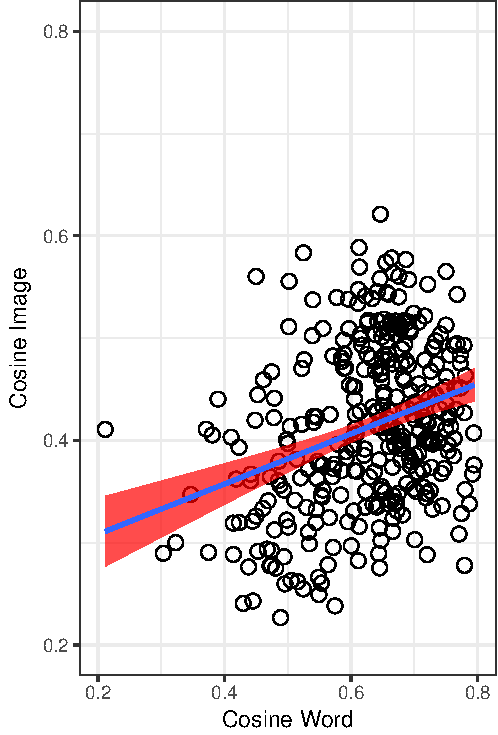
\includegraphics{figs/pairwise-corr-1} \caption[Relative cosine distance between points in word embedding space correlates with relative distance in image embedding space ($R = 0.30$, $p < 1.5e-08$)]{Relative cosine distance between points in word embedding space correlates with relative distance in image embedding space ($R = 0.30$, $p < 1.5e-08$). Graph contains all pairwise distances for every word.}\label{fig:pairwise-corr}
\end{figure}
\end{CodeChunk}

\begin{CodeChunk}
\begin{figure}[tb]
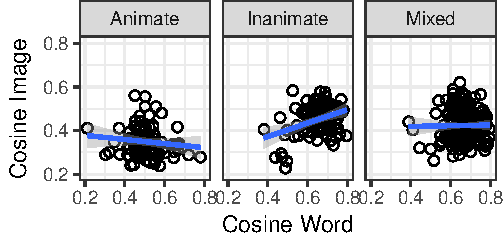
\includegraphics{figs/pairwise-corr-animate-vs-not-1} \caption[Inanimate objects display a significantly stronger correlation when mapping across vector spaces, meaning that they preserve their within-class structural relationships more reliabily across these two spaces]{Inanimate objects display a significantly stronger correlation when mapping across vector spaces, meaning that they preserve their within-class structural relationships more reliabily across these two spaces. Animate and mixed distances do not correlate. Each graph contains all pairwise distances between objects that are either a) both animate ($R = -0.13$, $p < 0.27$), b) both inanimate ($R = 0.38$, $p < 0.00024$), or c) mixed animate-to-inanimate ($R = -0.01$, $p < 0.86$)}\label{fig:pairwise-corr-animate-vs-not}
\end{figure}
\end{CodeChunk}

\begin{table}
\centering
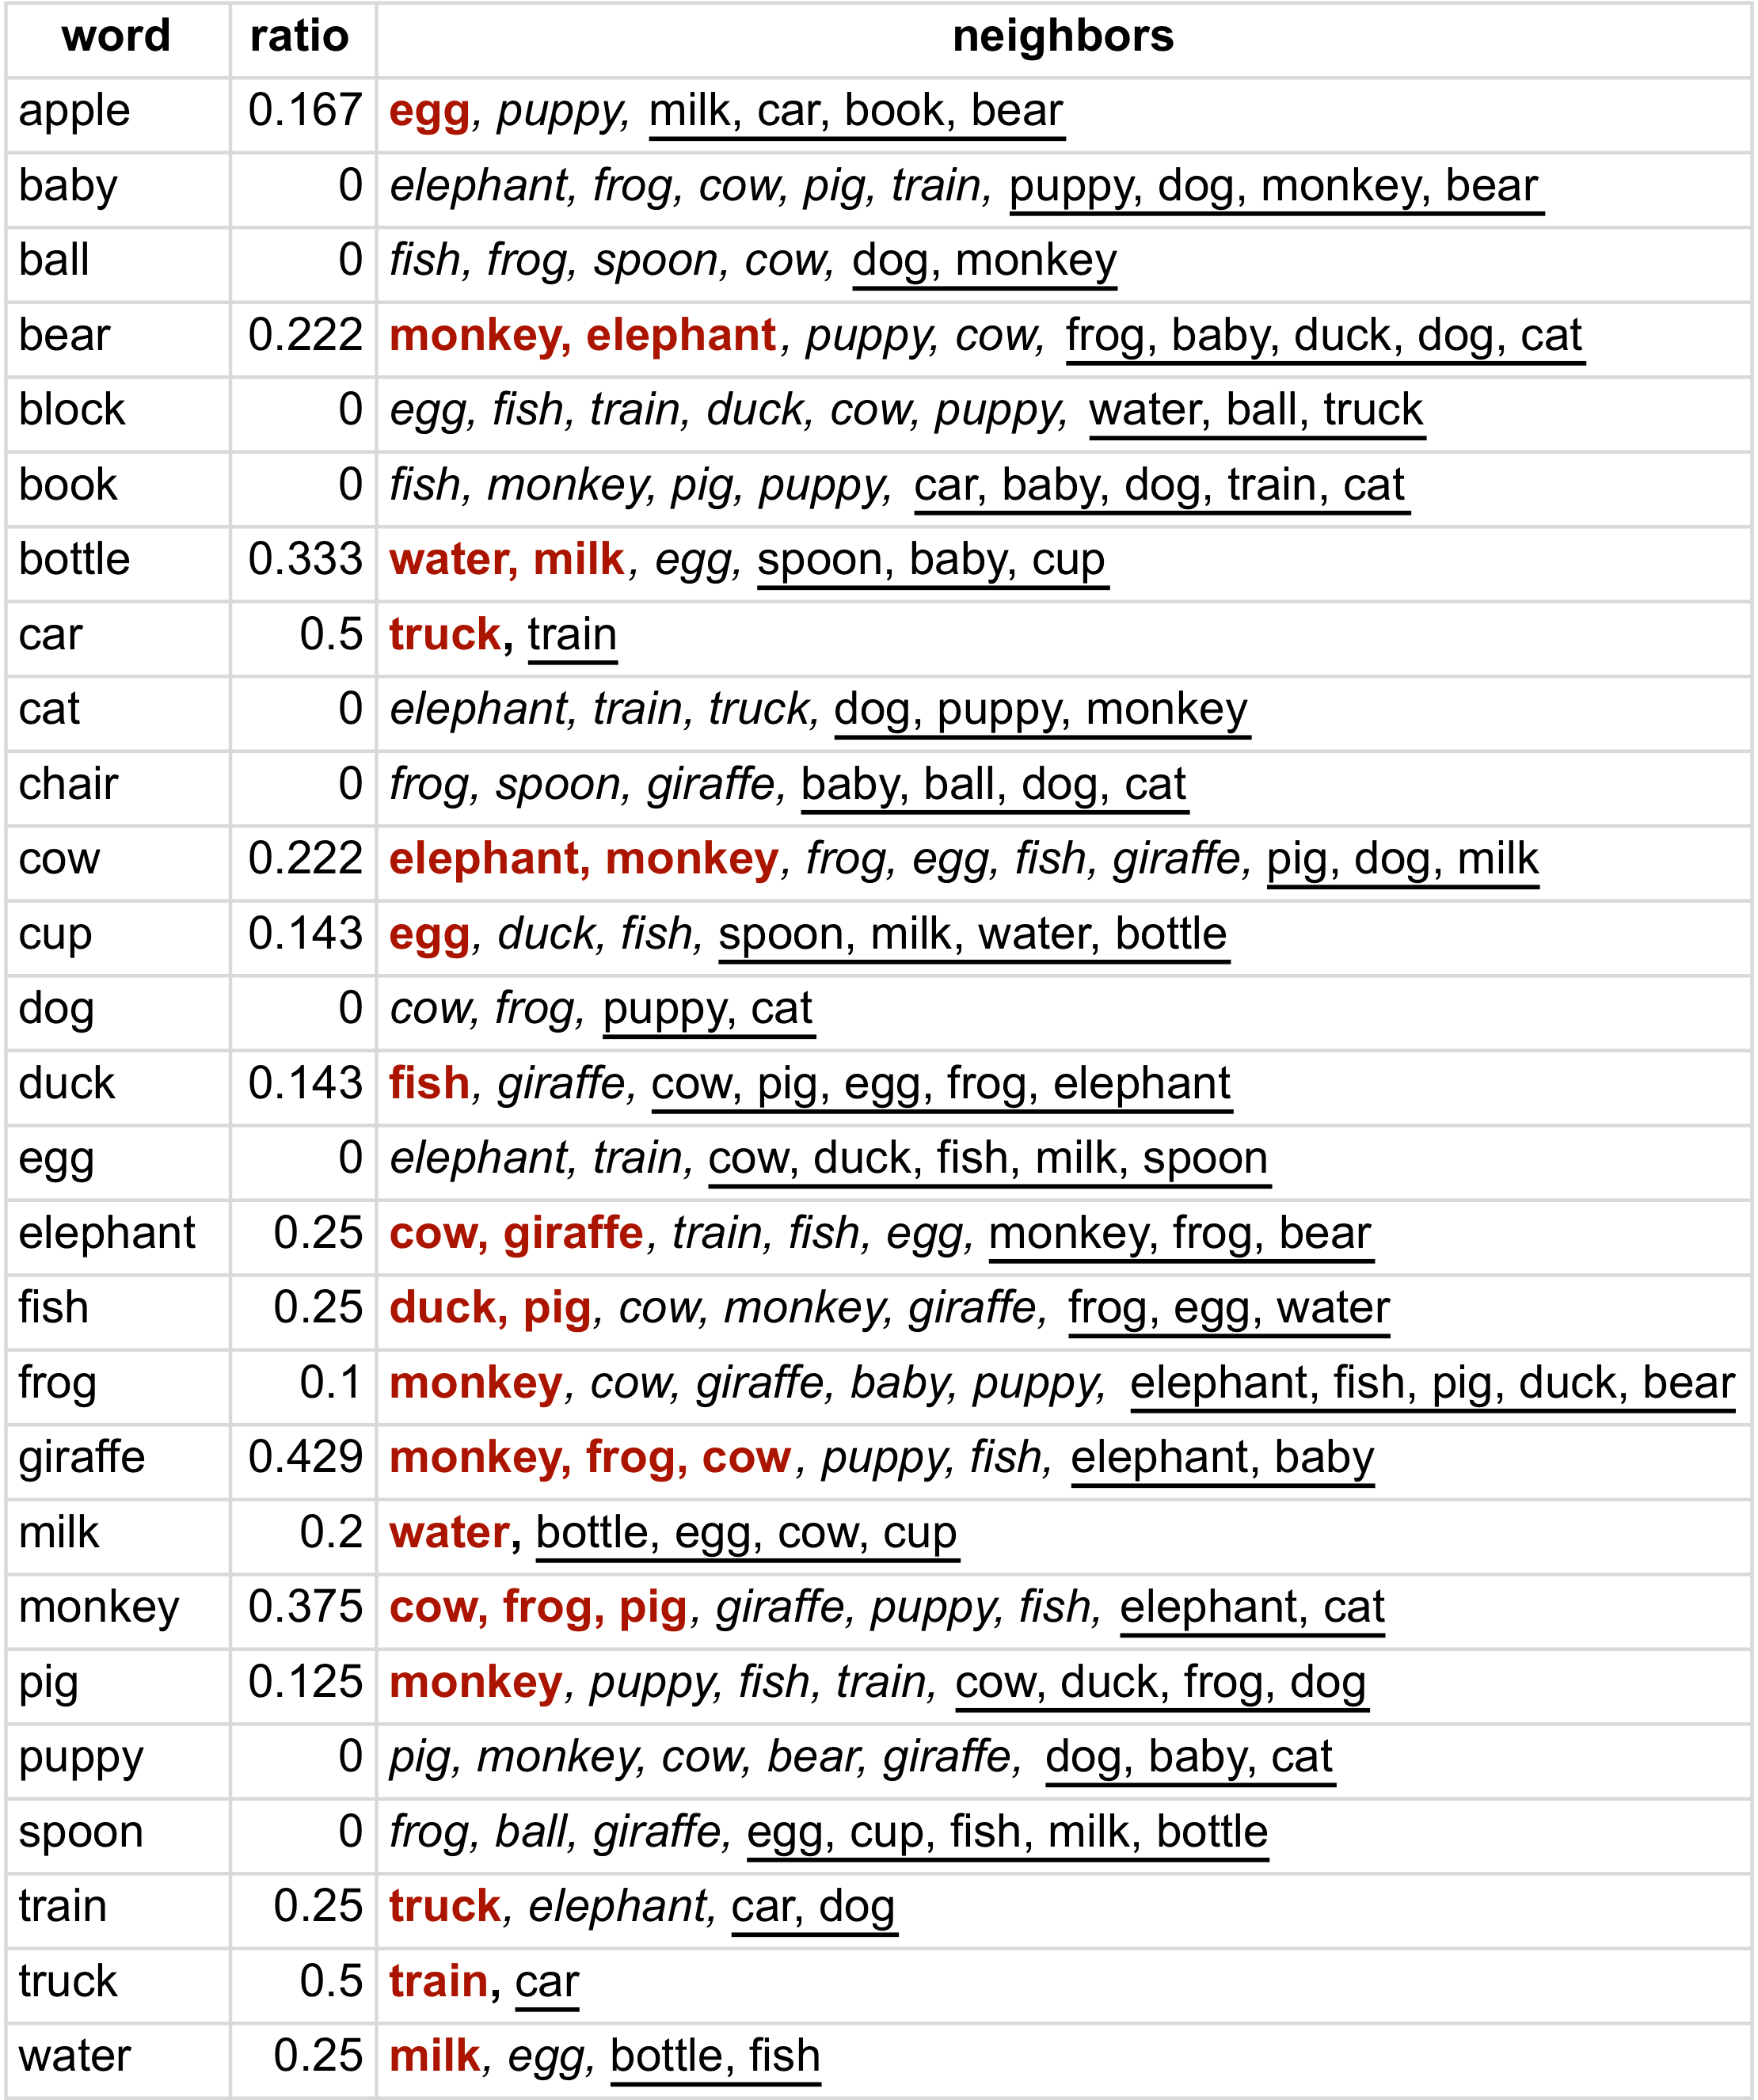
\includegraphics[max size={\columnwidth}{0.7\textheight}]{data/overlap_table_formatted2.png}
\caption{Overlaps between closest objects in image vector space and word vector space. Neighbors are defined as those other objects which are less than -1 SD from the mean distance for any given word. The overlap ratio is the number of shared neighbors across vector spaces divided by the total unique neighbors between the two spaces. Those neighbors that are marked red are shared between image and vector spaces. Italicized words only qualified as neighbors in the image space, while those that are underlined only qualify in the word space. Neighbors are sorted in increasing zcore order within their respective group (i.e. overlapping, just image, just word).}
\label{tbl:overlap-table}
\end{table}

\begin{CodeChunk}
\begin{figure}[tb]
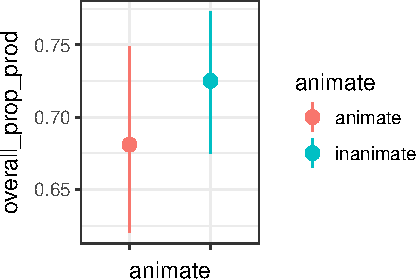
\includegraphics{figs/animacy-aoa-prod-graph-1} \caption[AoA for animates vs inanimates (using child production data) collapsed over month]{AoA for animates vs inanimates (using child production data) collapsed over month}\label{fig:animacy-aoa-prod-graph}
\end{figure}
\end{CodeChunk}

\begin{CodeChunk}
\begin{figure}[tb]
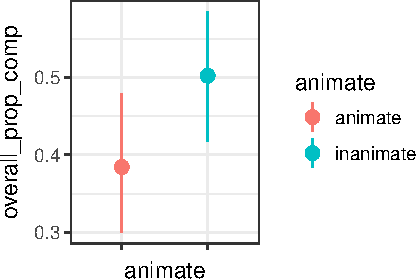
\includegraphics{figs/animacy-aoa-comp-graph-1} \caption[AoA for animates vs inanimates (using child comprehension data) collapsed over month]{AoA for animates vs inanimates (using child comprehension data) collapsed over month}\label{fig:animacy-aoa-comp-graph}
\end{figure}
\end{CodeChunk}

\section{\texorpdfstring{Discussion \textbf{Eb got to
here}}{Discussion Eb got to here}}\label{discussion-eb-got-to-here}

We've reported a significant correspondence between representations
learned by two different algorithms operating over seemingly unrelated
inputs (i.e.~visual and linguistic). What is most noteworthy here is
that the only immediate common ground between these representations are
the real life objects they both aim to model. This draws us into
questions concerning the nature of similarity and the multifaceted
character of information which is revealed by objects in the real world.
The notion that we can make inferences about one aspect of an object
given another aspect, is not surprising or controversial. However, the
fact that we can make these bi-directional inferences using aspects
traditionally treated as being orthogonal, is noteworthy. This is
particularly the case given the enormous dimensionality of our feature
spaces, and the fact that these algorithms are placed under no pressure
to find homologous representations.

Through what metrics can a learning algorithm, or indeed a human,
establish gradations of likeness? Are these necessarily the same metrics
which form the basis of category boundaries? These are fundamental
questions which have enjoyed a long history in the field (Edelman, 1998;
Hahn, Chater, \& Richardson, 2003; Kemp, Bernstein, \& Tenenbaum, 2005;
Shepard \& Chipman, 1970; Tversky, 1977). While our current work is not
sufficient to support a specific mechanism responsible for the observed
regularity, it might be indicative of the special role of invariance,
given that the unifying thread between our algorithms and inputs are the
common objects they represent. Underneath the diversity of visual
statistics and token distributions lie stable entities in the world
which, by virtue of their invariant actuality, give rise to regularity
across measurements at different vantage points (i.e.~modalities), an
idea dating back to Helmholtz (1878).

We find in our current work that this quality of invariance is
differentially present across different classes of entities, namely
animate vs.~inanimate objects. However, this is conditioned on the
particular algorithms we've investigated here, and our extensions into
human performance with our AoA anlysis did not show a significant
sensitivity to this difference. This could suggest a number things. The
first is that humans might not discover the regularities that these
algorithms do. Or it could be that our current class partitioning does
not provide sufficient contrast in invariance to register human AoA
differences. Or it could be that regularity is not a determining factor
in ease of acquisition. Of these three, the last is least likely to be
the case.

\section{Conclusion}\label{conclusion}

We find evidence of an interaction between visual and semantic features
learned by two distinct machine learning algorithms which operate over
drastically different inputs, and are trained in the service of
seemingly unrelated ends. This interaction is indicative of conserved
structure between these two supposedly independent sources of
information (i.e.~visual and functional). If humans are sensitive to
this relationship, as these algorithms seem to be, we expect that those
classes of object which are more strongly invariant across feature
spaces would be more easily learned by infants. We find a noticeable
though insignificant relationship between this property and AoA in our
current partitioning scheme (animates vs.~inanimates).

\section{Acknowledgements}\label{acknowledgements}

We thank the SEEDLingS team, and NIH DP5-OD019812.

\section{References}\label{references}

\setlength{\parindent}{-0.1in} \setlength{\leftskip}{0.125in} \noindent

\hypertarget{refs}{}
\hypertarget{ref-amatuni2017semantic}{}
Amatuni, A., \& Bergelson. (2017). Semantic networks generated from
early linguistic input. In \emph{Proceedings of the 39th annual
conference of the cognitive science society} (pp. 1538--1543).

\hypertarget{ref-bergelson2016seedlings}{}
Bergelson, E. (2016a). Bergelson seedlings homebank corpus.
\url{http://doi.org/10.21415/T5PK6D}

\hypertarget{ref-bergelson2016seedlingsdatabrary}{}
Bergelson, E. (2016b). SEEDLingS corpus. Retrieved January 26, 2018,
from \url{https://nyu.databrary.org/volume/228}

\hypertarget{ref-brent2001role}{}
Brent, M. R., \& Siskind, J. M. (2001). The role of exposure to isolated
words in early vocabulary development. \emph{Cognition}, \emph{81}(2),
B33--B44.

\hypertarget{ref-dale1996lexical}{}
Dale, P. S., \& Fenson, L. (1996). Lexical development norms for young
children. \emph{Behavior Research Methods, Instruments, \& Computers},
\emph{28}(1), 125--127.

\hypertarget{ref-edelman1998representation}{}
Edelman, S. (1998). Representation is representation of similarities.
\emph{Behavioral and Brain Sciences}, \emph{21}(4), 449--467.

\hypertarget{ref-firth1957synopsis}{}
Firth, J. R. (1957). A synopsis of linguistic theory, 1930-1955.
\emph{Studies in Linguistic Analysis}.

\hypertarget{ref-frank2017wordbank}{}
Frank, M. C., Braginsky, M., Yurovsky, D., \& Marchman, V. A. (2017).
Wordbank: An open repository for developmental vocabulary data.
\emph{Journal of Child Language}, \emph{44}(3), 677--694.

\hypertarget{ref-frank2009development}{}
Frank, M. C., Vul, E., \& Johnson, S. P. (2009). Development of infants'
attention to faces during the first year. \emph{Cognition},
\emph{110}(2), 160--170.

\hypertarget{ref-gelman1986categories}{}
Gelman, S. A., \& Markman, E. M. (1986). Categories and induction in
young children. \emph{Cognition}, \emph{23}(3), 183--209.

\hypertarget{ref-hahn2003similarity}{}
Hahn, U., Chater, N., \& Richardson, L. B. (2003). Similarity as
transformation. \emph{Cognition}, \emph{87}(1), 1--32.

\hypertarget{ref-harris1954distributional}{}
Harris, Z. S. (1954). Distributional structure. \emph{Word},
\emph{10}(2-3), 146--162.

\hypertarget{ref-helmholtz1878facts}{}
Helmholtz, H. (1878). The facts of perception. \emph{Selected Writings
of Hermann Helmholtz}, 1--15.

\hypertarget{ref-james2013principles}{}
James, W. (1890). \emph{The principles of psychology}. Henry Holt;
Company.

\hypertarget{ref-kemp2005generative}{}
Kemp, C., Bernstein, A., \& Tenenbaum, J. B. (2005). A generative theory
of similarity. In \emph{Proceedings of the 27th annual conference of the
cognitive science society} (pp. 1132--1137).

\hypertarget{ref-mandler2000perceptual}{}
Mandler, J. M. (2000). Perceptual and conceptual processes in infancy.
\emph{Journal of Cognition and Development}, \emph{1}(1), 3--36.

\hypertarget{ref-mareschal2001categorization}{}
Mareschal, D., \& Quinn, P. C. (2001). Categorization in infancy.
\emph{Trends in Cognitive Sciences}, \emph{5}(10), 443--450.

\hypertarget{ref-pennington2014glove}{}
Pennington, J., Socher, R., \& Manning, C. (2014). Glove: Global vectors
for word representation. In \emph{Proceedings of the 2014 conference on
empirical methods in natural language processing (emnlp)} (pp.
1532--1543).

\hypertarget{ref-quinn1997reexamination}{}
Quinn, P. C., \& Eimas, P. D. (1997). A reexamination of the
perceptual-to-conceptual shift in mental representations. \emph{Review
of General Psychology}, \emph{1}(3), 271.

\hypertarget{ref-quinn2000emergence}{}
Quinn, P. C., \& Eimas, P. D. (2000). The emergence of category
representations during infancy: Are separate perceptual and conceptual
processes required? \emph{Journal of Cognition and Development},
\emph{1}(1), 55--61.

\hypertarget{ref-quinn2000understanding}{}
Quinn, P. C., Johnson, M. H., Mareschal, D., Rakison, D. H., \& Younger,
B. A. (2000). Understanding early categorization: One process or two?
\emph{Infancy}, \emph{1}(1), 111--122.

\hypertarget{ref-ILSVRC15}{}
Russakovsky, O., Deng, J., Su, H., Krause, J., Satheesh, S., Ma, S.,
\ldots{} Fei-Fei, L. (2015). ImageNet Large Scale Visual Recognition
Challenge. \emph{International Journal of Computer Vision (IJCV)},
\emph{115}(3), 211--252. \url{http://doi.org/10.1007/s11263-015-0816-y}

\hypertarget{ref-shepard1970second}{}
Shepard, R. N., \& Chipman, S. (1970). Second-order isomorphism of
internal representations: Shapes of states. \emph{Cognitive Psychology},
\emph{1}(1), 1--17.

\hypertarget{ref-szegedy2016rethinking}{}
Szegedy, C., Vanhoucke, V., Ioffe, S., Shlens, J., \& Wojna, Z. (2016).
Rethinking the inception architecture for computer vision. In
\emph{Proceedings of the ieee conference on computer vision and pattern
recognition} (pp. 2818--2826).

\hypertarget{ref-trauble2007role}{}
Träuble, B., \& Pauen, S. (2007). The role of functional information for
infant categorization. \emph{Cognition}, \emph{105}(2), 362--379.

\hypertarget{ref-tversky1977features}{}
Tversky, A. (1977). Features of similarity. \emph{Psychological Review},
\emph{84}(4), 327.

\end{document}
